\documentclass[a4paper,12pt]{article}
\usepackage[fontsize=12pt]{fontsize}
\renewcommand{\baselinestretch}{1.25} 

\usepackage[margin=1in]{geometry}

\usepackage[utf8]{vietnam}
% \usepackage[vietnamese]{babel} 

\usepackage[dvipsnames, table]{xcolor} % for coloring
\usepackage{amsmath} % extension for math environment
\usepackage{bm} % bold math symbol
\usepackage{fancyvrb} % fancy verbatim
\usepackage{fvextra} % fancy verbatim extra
    \fvset{breaklines=true}

\usepackage[skip=.5em]{caption} % adjust spacing between figure and caption
\usepackage{subcaption}

% \usepackage[pdftex]{graphicx}
% \usepackage{url} 
\usepackage[bookmarks, 
    colorlinks=false, 
    pdfborder={0 0 0}, 
    pdftitle={Báo cáo BTL Thông tin di động}, 
    pdfauthor={Phạm Khánh}
]{hyperref} 

\usepackage{tikz} 
\usetikzlibrary{calc} % for drawing rectangle box at the cover

% FOR TABLE:
\usepackage{tabularx}
    \newcolumntype{L}[1]{>{\raggedright\arraybackslash}p{#1\textwidth}}
    \newcolumntype{C}[1]{>{\centering\arraybackslash}p{#1\textwidth}}
    \newcolumntype{R}[1]{>{\raggedleft\arraybackslash}p{#1\textwidth}
} % custom table environment
\usepackage{multirow}
\renewcommand{\arraystretch}{1.2}
\usepackage{longtable}

\usepackage{enumitem} % adjusting enum and itemize environment
    \setlist[itemize]{itemsep=0pt, topsep=3pt} % no item separation
    \setlist[enumerate]{itemsep=0pt, topsep=3pt} 
\usepackage{float} % forcing figure environment to be placed at an exact location

\setlength{\parskip}{0.5em} % spacing between paragraphs
\setlength\parindent{0pt} % do not indent the first paragraph

\usepackage{listings} % for embedding code
\lstset{frame=tb,
  aboveskip=5mm,
  belowskip=5mm,
  showstringspaces=false,
  columns=flexible,
  % basicstyle={\small\ttfamily},
  basicstyle={\ttfamily},
  lineskip={.1em}, % in case line spacing is too wide
  % numbers=none,
  numberstyle=\tiny\color{blue},
  keywordstyle=\color{red},
  commentstyle=\color{pink},
  stringstyle=\color{green},
  breaklines=true,
  breakatwhitespace=true,
  tabsize=4, 
  numbers=left,
  frame=single
}

\usepackage{biblatex}
\addbibresource{refs.bib}

\begin{document}
\renewcommand\bibname{Tài liệu tham khảo} 
\renewcommand{\listfigurename}{Danh sách hình minh họa}

\begin{titlepage}
    \begin{tikzpicture}[remember picture, overlay]
        \draw[line width = 4pt] ($(current page.north west) + (.75in,-.75in)$) rectangle ($(current page.south east) + (-.75in,.75in)$);
    \end{tikzpicture}
    
    \begin{center}
    	\textbf{ĐẠI HỌC QUỐC GIA THÀNH PHỐ HỒ CHÍ MINH}\\[3pt]
    	\textbf{TRƯỜNG ĐẠI HỌC BÁCH KHOA}\\ 
    	
    	\vspace{1.5cm}
    	
\includegraphics[width=4cm]{images/logo_BK.png}
    	\vspace{0.5cm}
    \end{center}
    
    \begin{center}
        \setlength{\parskip}{.5em}
        \par\noindent\rule{0.8\textwidth}{0.4pt}

        \textbf{{MÔN HỌC: THÔNG TIN DI ĐỘNG (EE5019)}}
        
        \textbf{{\large BÁO CÁO BÀI TẬP LỚN}}
    	    
        \textbf{{ƯỚC LƯỢNG KÊNH TRUYỀN VÔ TUYẾN}}
        \par\noindent\rule{0.8\textwidth}{0.4pt}
    \end{center}
    
    \vspace{1em}
    \begin{center}
        \renewcommand{\arraystretch}{1.5}
        \begin{tabular}{R{0.35} L{0.3} L{0.25}}
            \textbf{Giảng viên hướng dẫn:} & PGS. TS. Hà Hoàng Kha\\
            \textbf{Sinh viên thực hiện:} & Phạm Khánh & MSSV: 2011391\\
            & Lê Nguyên Khôi & MSSV: \\
            \textbf{Nhóm} & P01 -- Nhóm 2 & 
        \end{tabular}
    \end{center}
    
    \vfill
    \begin{center}
        Tp. Hồ Chí Minh -- 2024
    \end{center}
    \vspace{1em}
\end{titlepage}

\pagenumbering{roman}
\tableofcontents

\newpage
\pagenumbering{arabic} 

\section{Giới thiệu tổng quan}

Trong các hệ thống thông tin vô tuyến, kênh truyền đóng vai trò quan trọng do tín hiệu truyền qua kênh thường bị méo bởi các hiệu ứng như nhiễu, fading (suy hao), và tán xạ. 
Để khôi phục được tín hiệu đã truyền, đầu thu cần phải ước lượng kênh (channel estimation), tức là xác định đặc tính của kênh truyền để bù đắp sự méo dạng của tín hiệu. 
Việc ước lượng kênh hiệu quả giúp cải thiện chất lượng tín hiệu thu được và tăng cường hiệu suất của hệ thống truyền thông.

Ước lượng kênh thường được thực hiện bằng cách sử dụng các ký tự pilot - các tín hiệu đã biết trước, 
được chèn vào trong khung thời gian hoặc tần số. 
Dựa trên các giá trị pilot nhận được, hệ thống sẽ tính toán để ước lượng đặc tính của kênh tại các vị trí khác.

Các phương pháp ước lượng kênh phổ biến có thể kể đến là:

\begin{enumerate}
    \item \textbf{Least Squares (LS)}: Phương pháp đơn giản, chỉ sử dụng các ký tự pilot mà không cần thông tin thống kê của kênh. Tuy nhiên, độ chính xác không cao trong các môi trường có nhiễu.

    \item \textbf{Minimum Mean Square Error (MMSE)}: Sử dụng thông tin thống kê của kênh để cải thiện độ chính xác so với LS, nhưng có độ phức tạp tính toán cao và yêu cầu thông tin đầy đủ về kênh.

    \item \textbf{Phương pháp dựa trên học sâu (Deep Learning)}: Gần đây, các phương pháp ước lượng kênh dựa trên học sâu được phát triển, tận dụng các mạng nơ-ron để tự động học và ước lượng kênh từ dữ liệu. 
    Phương pháp này hứa hẹn hiệu suất cao hơn trong các môi trường phức tạp và nhiễu mạnh, nhưng yêu cầu quá trình huấn luyện mô hình phức tạp.
\end{enumerate}

Ước lượng kênh truyền vô tuyến đóng vai trò quan trọng trong nhiều ứng dụng thực tế, đặc biệt là trong các hệ thống truyền thông không dây. Một trong những ứng dụng phổ biến nhất là trong mạng di động như LTE (4G) và 5G NR. Trong các hệ thống này, ước lượng kênh được sử dụng để xử lý tín hiệu tại các trạm gốc và thiết bị đầu cuối, giúp đảm bảo truyền dữ liệu với độ chính xác cao, từ đó cải thiện chất lượng cuộc gọi, tốc độ truyền tải dữ liệu, và giảm thiểu hiện tượng mất gói tin.

Bên cạnh đó, ước lượng kênh cũng rất quan trọng trong hệ thống Wi-Fi, đặc biệt với các chuẩn Wi-Fi tiên tiến như Wi-Fi 6 và Wi-Fi 7. Nó giúp điều chỉnh quá trình truyền tải dữ liệu qua các băng tần cao, đảm bảo kết nối nhanh và ổn định hơn, đồng thời giảm nhiễu và tăng cường hiệu suất mạng. Điều này đặc biệt hữu ích trong các môi trường nhiều thiết bị kết nối như văn phòng hoặc nhà thông minh.

Trong các hệ thống liên lạc vệ tinh, ước lượng kênh giúp tối ưu hóa tín hiệu khi truyền qua khoảng cách xa và qua các môi trường khắc nghiệt như không gian và bầu khí quyển. Nhờ đó, tín hiệu truyền từ vệ tinh đến các trạm mặt đất hoặc ngược lại có thể được phục hồi chính xác, đảm bảo truyền tải dữ liệu an toàn và tin cậy, đặc biệt là trong các ứng dụng điều khiển từ xa hay viễn thám.

Trong lĩnh vực giao tiếp giữa các phương tiện, ước lượng kênh hỗ trợ mạnh mẽ cho hệ thống V2X (Vehicle-to-Everything), bao gồm giao tiếp giữa các phương tiện với nhau (V2V) hoặc giữa phương tiện và hạ tầng (V2I). Với tốc độ cao và điều kiện môi trường thay đổi liên tục, việc ước lượng kênh chính xác giúp đảm bảo truyền thông ổn định và kịp thời, tăng cường an toàn giao thông và hỗ trợ các hệ thống xe tự lái.

Một ứng dụng quan trọng khác là trong các hệ thống MIMO (Multiple Input Multiple Output), đặc biệt với 5G. Trong các hệ thống này, việc sử dụng nhiều anten để truyền tải và nhận tín hiệu yêu cầu một mô hình ước lượng kênh hiệu quả để tối ưu hóa băng thông và tốc độ truyền dữ liệu. Ước lượng kênh giúp hệ thống khai thác hiệu quả sự đa dạng của các kênh vô tuyến mà không tăng thêm yêu cầu về băng thông.

Ngoài ra, ước lượng kênh còn có ứng dụng trong các hệ thống radar và truyền thông quân sự, nơi tín hiệu phải đi qua những điều kiện môi trường phức tạp và bị nhiễu. Ước lượng kênh giúp tăng độ chính xác trong việc tái tạo tín hiệu, từ đó cung cấp thông tin liên lạc đáng tin cậy và an toàn trong các nhiệm vụ quân sự hoặc do thám.

Cuối cùng, trong các hệ thống Internet vạn vật (IoT), ước lượng kênh giúp các thiết bị cảm biến không dây hoạt động hiệu quả hơn trong các môi trường có nhiều nhiễu và thay đổi nhanh chóng về điều kiện kênh. Điều này đặc biệt quan trọng với các ứng dụng truyền thông tầm xa như LoRa, giúp duy trì kết nối ổn định và tiết kiệm năng lượng trong các mạng lưới cảm biến diện rộng.

Như vậy, ước lượng kênh truyền vô tuyến không chỉ là một phần không thể thiếu của các hệ thống truyền thông hiện đại mà còn là yếu tố quyết định hiệu suất và độ tin cậy trong nhiều ứng dụng khác nhau, từ mạng di động, Wi-Fi, đến các lĩnh vực chuyên biệt như liên lạc vệ tinh và hệ thống IoT.
\section{Mô hình hệ thống}

Mô hình hệ thống ước lượng kênh truyền vô tuyến mô tả quá trình một thiết bị thu nhận ước lượng chính xác về đặc tính của kênh vô tuyến giữa máy phát và máy thu. Quá trình này giúp thiết bị bù đắp được các ảnh hưởng của môi trường truyền thông (như nhiễu, suy hao, tán xạ) để tái tạo lại tín hiệu gốc. 

\subsection{Mô hình kênh vô tuyến}

Kênh truyền vô tuyến có thể được mô tả bằng phương trình đầu vào – đầu ra như sau:

\begin{equation}
    \bm{Y} = \bm{H} \cdot \bm{X} + \bm{N}
\end{equation}

Trong đó:
\begin{itemize}
    \item $\bm{Y}$: Tín hiệu nhận được tại thiết bị thu.
    \item $\bm{X}$: Tín hiệu đã truyền đi từ máy phát.
    \item $\bm{H}$: Ma trận kênh vô tuyến biểu diễn đặc tính của kênh (suy hao, trễ, tán xạ).
    \item $\bm{N}$: Nhiễu trắng Gaussian cộng (AWGN), mô tả nhiễu ảnh hưởng đến tín hiệu.
\end{itemize}

$\bm{H}$ là yếu tố cần được ước lượng chính xác để thiết bị thu có thể bù trừ các tác động của kênh và khôi phục lại $\bm{X}$ từ tín hiệu thu được $\bm{Y}$. 
Thông thường, kênh vô tuyến thay đổi theo thời gian và không gian, do đó việc ước lượng kênh đòi hỏi phải liên tục cập nhật trong suốt quá trình truyền dẫn.

\subsection{Ký tự pilot}

Ký tự pilot là các tín hiệu đã biết được chèn vào khung thời gian hoặc tần số của tín hiệu truyền để hỗ trợ ước lượng kênh. 
Các ký tự này được chèn vào với khoảng cách đã xác định trong cả miền thời gian và tần số (như trong hệ thống OFDM). 
Khi thiết bị thu nhận được các ký tự này, nó có thể sử dụng chúng để ước lượng các tham số của kênh tại những vị trí đã xác định, sau đó nội suy ra các vị trí khác.

Các cấu trúc chèn ký tự pilot thông thường gồm:

\begin{itemize}
    \item \textbf{Block-type}: Chèn pilot ở tất cả các subcarrier tại một vài khung thời gian.
    \item \textbf{Comb-type}: Chèn pilot vào một số subcarrier nhất định trong tất cả các khung thời gian.
    \item \textbf{Lattice-type}: Pilot được chèn vào theo mô hình hình học (như lưới) trong cả hai miền thời gian và tần số.
\end{itemize}
\subsection{Ước lượng kênh bằng LS}

Phương pháp ước lượng Least Squares (LS) là một trong những phương pháp đơn giản và phổ biến nhất để ước lượng kênh trong hệ thống thông tin vô tuyến. 
Mặc dù độ chính xác của nó không cao bằng các phương pháp khác như MMSE, nhưng LS có ưu điểm về tính đơn giản và không yêu cầu thông tin thống kê của kênh, điều này làm cho nó trở nên hiệu quả trong các ứng dụng không đòi hỏi hiệu suất tối ưu hoặc có giới hạn về tài nguyên tính toán.

\subsubsection{Mục tiêu của ước lượng LS}

Ý tưởng cơ bản của phương pháp LS là tìm ra ma trận kênh $\bm{\hat{H}}$ 
sao cho sai số giữa tín hiệu nhận được $\bm{y_p}$ và tín hiệu truyền đi $\bm{x_p}$, 
sau khi đi qua kênh, là nhỏ nhất. 
Trong thực tế, tín hiệu pilot \( \bm{x_p} \) được chèn vào một số vị trí đã biết trong khung thời gian-tần số để hỗ trợ ước lượng kênh. 
Phương pháp này dựa trên việc tối thiểu hóa sai số bình phương giữa tín hiệu thu nhận được và tín hiệu dự đoán (dựa trên mô hình kênh truyền và các ký tự pilot đã biết).

Tại các vị trí có ký tự pilot, giả sử mô hình kênh truyền được biểu diễn dưới dạng:

\begin{equation}
    \bm{y_p} = \bm{\hat{H}} \cdot \bm{x} + \bm{n}
\end{equation}

Trong đó:
\begin{itemize}
    \item $\bm{y_p}$: Tín hiệu nhận được tại thiết bị thu.
    \item $\bm{x_p}$: Tín hiệu pilot đã biết được truyền đi từ máy phát.
    \item $\bm{\hat{H}}$: Ma trận kênh vô tuyến cần được ước lượng.
    \item $\bm{n}$: Nhiễu trắng Gaussian cộng (AWGN), mô tả nhiễu ảnh hưởng đến tín hiệu.
\end{itemize}

\begin{figure}[H]
    \centering
    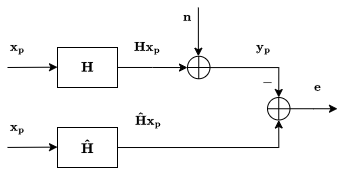
\includegraphics[width=0.65\linewidth]{../images/ls_block_diagram.png}
    \caption{Sơ đồ khối cho bộ ước lượng sai số bình phương tối thiểu}
\end{figure}

Mục tiêu của phương pháp ước lượng sai số bình phương tối thiểu là tìm một ma trận kênh truyền ước lượng \( \hat{\bm{H}} \) 
sao cho nó \textbf{giảm thiểu sai số bình phương} giữa tín hiệu thu thực tế \( \bm{y_p} \) và tín hiệu thu mong đợi \( \bm{\hat{H}} \bm{x_p} \). 
Sai số bình phương này có thể được định nghĩa qua hàm mất mát (loss function) như sau:

\[
\bm{J(\hat{H})} = \bm{e_1}^2 + \bm{e_2}^2 + ... + \bm{e_K}^2
\]
% 
\begin{equation}
    \bm{J(\hat{H})} = \| \bm{e} \|^2 = \| \bm{y_p} - \bm{\hat{H}}\bm{x_p} \|^2
\end{equation}

Trong đó:
\begin{itemize}
    \item \( \bm{y_p} - \bm{\hat{H}}\bm{x_p} \) là sai số giữa tín hiệu thu thực tế và tín hiệu thu mong đợi
    \item \( \|\cdot\|^2 \) là chuẩn bình phương Euclidean, đại diện cho tổng bình phương sai số giữa các phần tử của vector
\end{itemize}

Để tối thiểu hóa sai số bình phương, ta cần tìm ma trận kênh truyền \( \hat{\mathbf{H}} \) tối ưu. Điều này được thực hiện bằng cách giải phương trình tối ưu hóa sau:
%
\begin{equation}
    \bm{\hat{H}} 
    = \underset{\bm{\hat{H}}}{\arg \min} \; \bm{J(\hat{H})}
    = \underset{\bm{\hat{H}}}{\arg \min} \; \|\bm{y_p} - \bm{\hat{H}}\bm{x_p}\|^2
\end{equation}

\subsubsection{Tìm nghiệm tối ưu của ước lượng LS}

Trước hết, ta triển khai hàm mất mát \( \bm{J(\hat{H})} \): 
% 
\begin{align*}
    \bm{J(\hat{H})} 
    &= \| \bm{y_p} - \bm{\hat{H}}\bm{x_p} \|^2 \\
    &= (\bm{y_p} - \bm{\hat{H}}\bm{x_p})^H (\bm{y_p} - \bm{\hat{H}}\bm{x_p}) \\
    &= (\bm{y_p}^H - \bm{x_p}^H\bm{\hat{H}}^H) (\bm{y_p} - \bm{\hat{H}}\bm{x_p}) \\
    &= \bm{y_p}^H\bm{y_p} - \bm{y_p}^H\bm{\hat{H}}\bm{x_p} - \bm{x_p}^H\bm{\hat{H}}^H\bm{y_p} + \bm{x_p}^H\bm{\hat{H}}^H\bm{\hat{H}}\bm{x_p}
\end{align*}

Nghiệm tối ưu của phương pháp Least Squares có thể tìm được bằng cách cho gradient của hàm mất mát theo vector \( \bm{\hat{x}} \) bằng không:
% 
\begin{align*}
    \nabla_{\bm{\hat{H}}}\bm{J(\hat{H})}
    &= - \bm{y_p}\bm{x_p}^H + \bm{\hat{H}}\bm{x_p}\bm{x_p}^H = 0\\
    &\Leftrightarrow \bm{\hat{H}}\bm{x_p} = \bm{y_p}
\end{align*}

Vậy nghiệm tối ưu của kênh truyền ước lượng theo phương pháp LS là:
% 
\begin{equation}
    \bm{\hat{H}} = \bm{y_p}\bm{x_p}^H
\end{equation}

\textbf{Nhận xét}

Phương pháp Least Squares (LS) trong ước lượng kênh truyền vô tuyến có ưu điểm nổi bật là đơn giản và dễ triển khai. 
Phương pháp này không yêu cầu kiến thức sâu về thống kê hay xử lý tín hiệu, 
do đó rất phù hợp với các hệ thống có tài nguyên hạn chế. 
Hơn nữa, LS không cần thông tin về phân phối hay đặc tính của nhiễu, 
chỉ sử dụng tín hiệu huấn luyện và tín hiệu nhận được để ước lượng kênh. 
Trong điều kiện kênh truyền có tỷ lệ tín hiệu trên nhiễu cao, 
phương pháp này có thể mang lại kết quả khá chính xác.  

Tuy nhiên, LS tồn tại một số hạn chế quan trọng. 
Đầu tiên, nó rất nhạy cảm với nhiễu, đặc biệt trong các môi trường có SNR thấp. 
Do không xem xét tác động của nhiễu, kết quả ước lượng của LS thường bị suy giảm nghiêm trọng khi nhiễu mạnh xuất hiện. 
Thêm vào đó, LS không phải là một phương pháp tối ưu về mặt thống kê; 
các phương pháp khác như Minimum Mean Square Error (MMSE) thường cho kết quả tốt hơn nhờ tận dụng được thông tin thống kê của nhiễu. 
Ngoài ra, hiệu quả của LS còn phụ thuộc lớn vào tín hiệu huấn luyện. 
Nếu tín hiệu này không đủ mạnh hoặc bị lỗi, ước lượng kênh có thể không chính xác.

Phương pháp LS thường được sử dụng trong các ứng dụng không đòi hỏi cao về độ chính xác hoặc trong giai đoạn sơ bộ của ước lượng kênh. 
Nó cũng có thể được dùng làm bước khởi tạo cho các phương pháp tiên tiến hơn như MMSE hay các thuật toán dựa trên máy học. 
Để cải thiện hiệu suất của LS, ta có thể tối ưu độ dài và công suất của tín hiệu huấn luyện.

Phương pháp LS, mặc dù đơn giản, vẫn là một công cụ hữu ích trong nhiều tình huống. Tuy nhiên, để đạt hiệu suất cao hơn, nó thường được kết hợp với các kỹ thuật tiên tiến khác.

\subsubsection{Nội suy để ước lượng kênh tại các vị trí không phải pilot}

Phương pháp LS chỉ ước lượng được ma trận kênh \( \bm{H} \) tại các vị trí có ký tự pilot. 
Để tính toán giá trị kênh tại các vị trí không có ký tự pilot, các phương pháp \textbf{nội suy hai chiều} (2D interpolation) sẽ được sử dụng. 
Một số phương pháp nội suy phổ biến bao gồm:

\begin{itemize}
    \item Nội suy tuyến tính (Linear interpolation),
    \item Nội suy spline,
    \item Nội suy bậc cao (Higher-order interpolation).
\end{itemize}

Nội suy giúp tạo ra một ma trận kênh ước lượng đầy đủ tại tất cả các vị trí trong khung thời gian và tần số, dựa trên thông tin từ các vị trí pilot.
\section{Giải pháp ước lượng kênh MMSE, LS, và máy học}

\subsection{Ước lượng kênh bằng MMSE}

Phương pháp Minimum Mean Square Error (MMSE) là một trong những phương pháp ước lượng kênh truyền tiên tiến, mang lại độ chính xác cao hơn so với Least Squares (LS) bằng cách sử dụng thông tin thống kê về kênh truyền và nhiễu. 
MMSE không chỉ giảm thiểu sai số giữa kênh ước lượng và kênh thực mà còn tối ưu hóa hiệu suất trong môi trường có nhiễu và fading mạnh. 

\subsubsection{Mục tiêu của ước lượng MMSE}

MMSE dựa trên việc tối thiểu hóa trung bình bình phương sai số (MSE) giữa kênh truyền thực tế và kênh ước lượng. 
Điều này có nghĩa là MMSE không chỉ dựa vào tín hiệu đã nhận mà còn sử dụng thông tin thống kê về kênh truyền và nhiễu, 
từ đó đưa ra ước lượng tốt hơn so với LS. 
Cụ thể, MMSE cố gắng tối thiểu hóa sai số kỳ vọng giữa kênh thực và kênh ước lượng bằng cách tìm ma trận lọc tối ưu.

Dựa trên kênh truyền đã được ước lượng bằng phương pháp LS:
% 
\begin{align*}
    \bm{\hat{H}_p} 
    &= \bm{y_p}\bm{x_p}^H \\
    &= (\bm{H_d}\bm{x_p} + \bm{n})\bm{x_p}^H \\
    &= \bm{H_d}\bm{x_p}\bm{x_p}^H + \bm{n}\bm{x_p}^H \\
    &= \bm{H_d} + \bm{n}\bm{x_p}^H
\end{align*}

Ta tiến hành nhân kênh truyền đã ước lượng LS với một ma trận lọc \( \bm{W} \):

\[
    \bm{\hat{H}} = \bm{W}\bm{\hat{H}_p} 
\]

\begin{figure}[H]
    \centering
    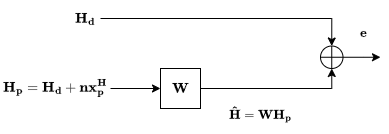
\includegraphics[width=.75\textwidth]{../images/mmse_block_diagram.png}
    \caption{Ước lượng kênh bằng phương pháp MMSE}
\end{figure}

Mục tiêu của phương pháp ước lượng MMSE là tìm ma trận lọc \( \bm{W} \) 
sao cho nó \textbf{giảm thiểu sai số bình phương trung bình} MSE giữa kênh truyền thực tế \( \bm{H_d} \) 
và kênh truyền ước lượng \( \bm{\hat{H}} = \bm{W}\bm{\hat{H}_p} \). 
MSE có thể được định nghĩa qua hàm mất mát (loss function) như sau:

\begin{equation}
    \bm{J(W)} 
    = \bb{E} \left[ \| \bm{e} \|^2 \right]
    = \bb{E} \left[ \| \bm{H_d} - \bm{W}\bm{\hat{H}_p} \|^2 \right]
\end{equation}

Trong đó, \( \bm{e} = \bm{H_d} - \bm{W}\bm{\hat{H}_p} \) là ma trận sai số giữa kênh thực tế và kênh ước lượng.

Để tối thiểu hóa MSE, ta cần tìm \( \bm{W} \) để tối thiểu hàm mất mát. 
Điều này được thực hiện bằng cách giải phương trình tối ưu hóa sau:
%
\begin{equation}
    \bm{W} 
    = \underset{\bm{W}}{\arg \min} \; \bm{J(W)}
    = \underset{\bm{W}}{\arg \min} \; \bb{E} \left[ \| \bm{H_d} - \bm{W}\bm{\hat{H}_p} \|^2 \right]
\end{equation}

\subsubsection{Tìm nghiệm tối ưu của ước lượng MMSE}

Dựa trên nguyên lý trực giao, ta có ma trận sai số \( \bm{e} \) trực giao với \( \bm{\hat{H}} \). 
Hơn nữa, \( \bm{\hat{H}} = \bm{W}\bm{\hat{H}_p} \) với \( \bm{W} \) là ma trận của một phép biến đổi tuyến tính, nên \( \bm{e} \) cũng trực giao với \( \bm{\hat{H}_p} \):

\begin{figure}[H]
    \centering
    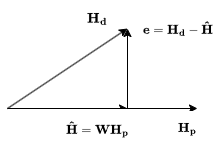
\includegraphics[width=.4\textwidth]{../images/mmse_orthogonal.png}
    \caption{Ma trận sai số \( \bm{e} \) trực giao với \( \bm{\hat{H}_p} \)}
\end{figure}

\begin{align*}
    \bb{E} \left[ \bm{e} \bm{\hat{H}_p}^H \right] 
    &= \bb{E} \left[ (\bm{H_d} - \bm{W}\bm{\hat{H}_p}) \bm{\hat{H}_p}^H \right] \\
    &= \bb{E} \left[ \bm{H_d}\bm{\hat{H}_p}^H - \bm{W}\bm{\hat{H}_p}\bm{\hat{H}_p}^H \right] \\
    &= \bb{E} \left[ \bm{H_d}\bm{\hat{H}_p}^H \right] - \bm{W}\bb{E} \left[ \bm{\hat{H}_p}\bm{\hat{H}_p}^H \right] \\
    &= \bm{R_{dp}} - \bm{W}\bm{R_{pp}} = 0
\end{align*}

Trong đó, \( \bm{R_{dp}} = \bb{E} \left[ \bm{H_d}\bm{\hat{H}_p}^H \right] \) là ma trận tương quan giữa kênh thực và kênh ước lượng, 
và \( \bm{R_{pp}} = \bb{E} \left[ \bm{\hat{H}_p}\bm{\hat{H}_p}^H \right] \) là ma trận tự tương quan của kênh ước lượng tại các vị trí pilot.

Từ đó, ta có:

\[
    \bm{W} = \bm{R_{dp}} \bm{R_{pp}}^{H}
\]

\( \bm{R_{pp}} \) được tính bởi:
% 
\begin{align*}
    \bm{R_{pp}} 
    &= \bb{E} \left[ \bm{\hat{H}_p}\bm{\hat{H}_p}^H \right] \\
    &= \bb{E} \left[ (\bm{H_d} + \bm{n}\bm{x_p}^H)(\bm{H_d} + \bm{n}\bm{x_p}^H)^H \right] \\
    &= \bb{E} \left[ \bm{H_d}\bm{H_d}^H + \bm{H_d}\bm{n}^H\bm{x_p} + \bm{n}\bm{x_p}^H\bm{H_d}^H + \bm{n}\bm{n}^H\bm{x_p}\bm{x_p}^H \right] \\
    &= \bm{R_{dd}} + \sigma_n^2\bm{x_p}\bm{x_p}^H
\end{align*}

Trong đó, \( \bm{R_{dd}} = \bb{E} \left[ \bm{H_d}\bm{H_d}^H \right] \) là ma trận tương quan của kênh thực tế. Thay vào phương trình trên, ta có:

\begin{equation}
    \bm{W} = \bm{R_{dp}} (\bm{R_{dd}} + \sigma_n^2\bm{x_p}\bm{x_p}^H)^{H}
\end{equation}

Phương pháp này dựa vào việc mô tả thống kê của kênh truyền và tín hiệu nhận được. 
Nếu các ma trận tương quan này được ước lượng chính xác, MMSE sẽ cho kết quả ước lượng kênh chính xác hơn đáng kể so với LS.

\subsubsection{Ước lượng kênh tại các vị trí không phải pilot}

Để ước lượng kênh tại các vị trí không phải pilot, phương pháp nội suy có thể được áp dụng. 
Do MMSE đã khai thác thông tin thống kê của kênh, kết quả nội suy thường chính xác hơn so với nội suy từ ước lượng LS.


\subsection{Ước lượng kênh bằng kĩ thuật học sâu}

Phương pháp ước lượng kênh truyền vô tuyến dựa trên kỹ thuật học sâu (Deep Learning - DL) đã nổi lên như một giải pháp tiên tiến trong các hệ thống thông tin không dây, 
đặc biệt trong bối cảnh các hệ thống ngày càng phức tạp như MIMO hay OFDM. 
Các kỹ thuật học sâu có khả năng tự động học mô hình và xử lý các vấn đề phi tuyến mà các phương pháp truyền thống như LS hay MMSE gặp khó khăn \cite{Soltani2019}. 

\subsubsection{Nguyên lý của ước lượng kênh dựa trên học sâu}

Phương pháp ước lượng kênh truyền dựa trên học sâu sử dụng mạng nơ-ron nhân tạo (Artificial Neural Networks - ANN) để học cách biểu diễn và dự đoán kênh truyền từ dữ liệu nhận được, 
thay vì dựa trên các mô hình thống kê hoặc các công thức toán học cố định như trong MMSE hoặc LS. 
Mục tiêu chính là học mối quan hệ giữa tín hiệu nhận được và kênh truyền, từ đó ước lượng đặc tính kênh một cách chính xác và tự động.

Kênh truyền có thể được coi như một bản đồ hai chiều (2D) trong miền thời gian và tần số. 
Ý tưởng của DL là mô hình hóa đáp ứng kênh truyền theo thời gian và tần số như một hình ảnh hai chiều và sử dụng các mạng nơ-ron tích chập để học cách ước lượng kênh từ dữ liệu đầu vào.

\subsubsection{Kiến trúc mạng học sâu cho ước lượng kênh}

Phương pháp học sâu cho ước lượng kênh có thể sử dụng nhiều loại kiến trúc khác nhau, nhưng phổ biến nhất là Mạng nơ-ron tích chập (CNN - Convolutional Neural Networks). 
CNN đặc biệt phù hợp cho việc xử lý dữ liệu dạng lưới như hình ảnh hoặc dữ liệu thời gian-tần số trong các hệ thống thông tin không dây.

\begin{table}[H]
    \centering
    \begin{tabular}{cccc}
        \hline
        \textbf{Thứ tự} & \textbf{Lớp} & \textbf{Kích thước ngõ ra} & \textbf{Số lượng tham số} \\
        \hline
        1 & Input & (số mẫu, 72, 14, 1) & 0 \\
        2 & Conv2D & (số mẫu, 72, 14, 64) & 5248 \\
        3 & Conv2D & (số mẫu, 72, 14, 32) & 2080 \\
        4 & Conv2D & (số mẫu, 72, 14, 1) & 801
    \end{tabular}
\end{table}

\subsubsection{Quy trình ước lượng kênh dựa trên học sâu}

Các bước chính trong quy trình ước lượng kênh dựa trên học sâu:

\textbf{Thu thập dữ liệu và tiền xử lý}

\begin{itemize}
    \item \textbf{Thu thập dữ liệu}: 
    Dữ liệu bao gồm các tín hiệu nhận được tại máy thu cùng với các thông tin pilot đã biết. 
    Các mẫu dữ liệu này sẽ được dùng để huấn luyện mô hình DL.
    \item \textbf{Chuẩn hóa dữ liệu}: 
    Dữ liệu phải được chuẩn hóa để phù hợp với đầu vào của mạng nơ-ron. 
    Ví dụ, dữ liệu có thể được chuẩn hóa về các phạm vi giá trị chuẩn để mô hình học dễ dàng hơn.
\end{itemize}

\textbf{Huấn luyện mô hình học sâu}

Mạng học sâu được huấn luyện trên dữ liệu từ kênh truyền để học cách ước lượng các giá trị kênh dựa trên các mẫu tín hiệu nhận được. 
Quá trình huấn luyện thường bao gồm:

\begin{itemize}
    \item \textbf{Xác định hàm mất mát}: Hàm mất mát thường được sử dụng là Mean Square Error (MSE) giữa kênh ước lượng và kênh thực, tức là:

    \begin{equation}
        \mathcal{L} = \frac{1}{N} \sum_{i=1}^{N} \| \bm{H_i} - \bm{\hat{H}_i} \|^2
    \end{equation}
    
    Trong đó \( \bm{H_i} \) là kênh thực và \( \bm{\hat{H}_i} \) là kênh ước lượng từ mạng nơ-ron.

    \item \textbf{Tối ưu hóa}: Để huấn luyện mạng nơ-ron, ta cần một tập dữ liệu lớn chứa các mẫu tín hiệu nhận được và kênh truyền tương ứng. Thuật toán tối ưu hóa được chọn là Adam với hàm mất mát là Mean Square Error (MSE) giữa kênh ước lượng và kênh thực. Tốc độ học (learning rate) được chọn là 0.001.
\end{itemize}

\textbf{Kiểm thử và đánh giá}

Sau khi huấn luyện, mô hình DL được kiểm thử trên một tập dữ liệu mới để đánh giá khả năng ước lượng kênh. 
Kết quả thường được so sánh với các phương pháp truyền thống như LS hoặc MMSE dựa trên các chỉ số như MSE hoặc Signal-to-Noise Ratio (SNR).
\section{Chương trình Python mô phỏng ước lượng kênh truyền}

File \verb|models.py| chứa các hàm phục vụ cho việc ước lượng kênh truyền vô tuyến bằng kỹ thuật học sâu, với hai mô hình chính là SRCNN và DnCNN.

Hàm \verb|psnr()| tính toán chỉ số PSNR (Peak Signal-to-Noise Ratio), 
dùng để đánh giá chất lượng hình ảnh tái tạo \verb|target| so với ảnh gốc \verb|ref|.
Công thức tính PSNR dựa trên căn sai số bình phương trung bình (RMSE) giữa hai ảnh, sau đó chuyển đổi sang dB:

\begin{lstlisting}[language=Python]
def psnr(target, ref):
    # assume RGB image
    target_data = np.array(target, dtype=float)
    ref_data = np.array(ref, dtype=float)

    diff = ref_data - target_data
    diff = diff.flatten('C')

    rmse = math.sqrt(np.mean(diff ** 2.))

    return 20 * math.log10(255. / rmse)
\end{lstlisting}

Hàm \verb|interpolation(noisy, snr, number_of_pilot, interp)| thực hiện nội suy tín hiệu nhận được dựa trên số lượng pilot đã chọn và phương pháp nội suy (RBF hoặc spline).
Hàm này tạo ra ảnh kênh truyền có độ phân giải cao bằng cách nội suy từ các giá trị pilot, sau đó trả về ảnh nội suy với kích thước tương ứng.

Hàm \verb|SRCNN_model()| tạo và trả về mô hình Super-Resolution Convolutional Neural Network (SRCNN). Mô hình bao gồm 3 lớp tích chập:
\begin{itemize}
    \item Lớp đầu tiên có 64 bộ lọc kích thước $9 \times 9$.
    \item Lớp thứ hai có 32 bộ lọc kích thước $1 \times 1$.
    \item Lớp cuối cùng có 1 bộ lọc kích thước $5 \times 5$.
\end{itemize}

Mô hình được biên dịch với hàm mất mát mean squared error (MSE) và được tối ưu bằng Adam.

\begin{lstlisting}[language=Python]
def SRCNN_model():
    input_shape = (72, 14, 1)
    x = Input(shape=input_shape)
    c1 = Conv2D(64, (9, 9), activation="relu", padding="same", kernel_initializer="he_normal")(x)
    c2 = Conv2D(32, (1, 1), activation="relu", padding="same", kernel_initializer="he_normal")(c1)
    c3 = Conv2D(1, (5, 5), padding="same", kernel_initializer="he_normal")(c2)
    # c4 = Input(shape = input_shape)(c3)
    model = Model(inputs=x, outputs=c3)
    # compile
    adam = Adam(learning_rate=0.001, beta_1=0.9, beta_2=0.999, epsilon=1e-8)
    model.compile(optimizer=adam, loss='mean_squared_error', metrics=['mean_squared_error'])
    return model
\end{lstlisting}

Hàm \verb|SRCNN_train()| huấn luyện mô hình SRCNN trên dữ liệu kênh truyền. 
Đầu tiên, hàm này gọi hàm \verb|SRCNN_model()| để tạo mô hình và sử dụng dữ liệu đầu vào để huấn luyện. 
Hàm này cũng sử dụng \verb|ModelCheckpoint| để lưu mô hình với kết quả tốt nhất dựa trên validation loss.

\begin{lstlisting}[language=Python]
def SRCNN_train(train_data, train_label, val_data, val_label, channel_model, num_pilots, SNR):
    srcnn_model = SRCNN_model()
    print(srcnn_model.summary())

    checkpoint = ModelCheckpoint("SRCNN_check.h5", monitor='val_loss', verbose=1, save_best_only=True,
                                 save_weights_only=False, mode='min')
    callbacks_list = [checkpoint]

    srcnn_model.fit(train_data, train_label, batch_size=128, validation_data=(val_data, val_label),
                    callbacks=callbacks_list, shuffle=True, epochs=300, verbose=0)

    srcnn_model.save_weights("SRCNN_" + channel_model + "_" + str(num_pilots) + "_" + str(SNR) + ".h5")
\end{lstlisting}

Hàm \verb|SRCNN_predict()| tải trọng số của mô hình SRCNN đã huấn luyện từ tệp và sử dụng mô hình để dự đoán dữ liệu đầu vào \verb|input_data|.

\begin{lstlisting}[language=Python]
def SRCNN_predict(input_data, channel_model, num_pilots, SNR):
    srcnn_model = SRCNN_model()
    srcnn_model.load_weights("SRCNN_" + channel_model + "_" + str(num_pilots) + "_" + str(SNR) + ".h5")
    predicted = srcnn_model.predict(input_data)
    return predicted
\end{lstlisting}

Hàm \verb|DNCNN_model()| tạo và trả về mô hình Denoising Convolutional Neural Network (DnCNN). 
Mô hình bao gồm:
\begin{itemize}
    \item Lớp tích chập đầu tiên với 64 bộ lọc $3 \times 3$ và hàm kích hoạt ReLU.
    \item 18 lớp tiếp theo gồm tích chập, batch normalization và ReLU.
    \item Lớp cuối cùng thực hiện phép trừ đầu vào với kết quả tích chập để loại bỏ nhiễu khỏi tín hiệu.
\end{itemize}

\begin{lstlisting}[language=Python]
def DNCNN_model():
    inpt = Input(shape=(None, None, 1))
    # 1st layer, Conv+relu
    x = Conv2D(filters=64, kernel_size=(3, 3), strides=(1, 1), padding='same')(inpt)
    x = Activation('relu')(x)
    # 18 layers, Conv+BN+relu
    for i in range(18):
        x = Conv2D(filters=64, kernel_size=(3, 3), strides=(1, 1), padding='same')(x)
        x = BatchNormalization(axis=-1, epsilon=1e-3)(x)
        x = Activation('relu')(x)
        # last layer, Conv
    x = Conv2D(filters=1, kernel_size=(3, 3), strides=(1, 1), padding='same')(x)
    x = Subtract()([inpt, x])  # input - noise
    model = Model(inputs=inpt, outputs=x)
    adam = Adam(learning_rate=0.001, beta_1=0.9, beta_2=0.999, epsilon=1e-8)
    model.compile(optimizer=adam, loss='mean_squared_error', metrics=['mean_squared_error'])
    return model
\end{lstlisting}

Hàm \verb|DNCNN_train()| huấn luyện mô hình DnCNN trên dữ liệu kênh truyền và lưu lại mô hình tốt nhất. 
Quy trình tương tự như hàm huấn luyện cho SRCNN, với một checkpoint để lưu mô hình tốt nhất dựa trên validation loss.

\begin{lstlisting}[language=Python]
def DNCNN_train(train_data, train_label, val_data, val_label, channel_model, num_pilots, SNR):
    dncnn_model = DNCNN_model()
    print(dncnn_model.summary())

    checkpoint = ModelCheckpoint("DNCNN_check.h5", monitor='val_loss', verbose=1, save_best_only=True,
                                 save_weights_only=False, mode='min')
    callbacks_list = [checkpoint]

    dncnn_model.fit(train_data, train_label, batch_size=128, validation_data=(val_data, val_label),
                    callbacks=callbacks_list, shuffle=True, epochs=200, verbose=0)
    dncnn_model.save_weights("DNCNN_" + channel_model + "_" + str(num_pilots) + "_" + str(SNR) + ".h5")
\end{lstlisting}

Hàm \verb|DNCNN_predict()| tải mô hình DnCNN đã được huấn luyện và sử dụng để dự đoán trên dữ liệu đầu vào \verb|input_data|.

\begin{lstlisting}[language=Python]
def DNCNN_predict(input_data, channel_model, num_pilots, SNR):
    dncnn_model = DNCNN_model()
    dncnn_model.load_weights("DNCNN_" + channel_model + "_" + str(num_pilots) + "_" + str(SNR) + ".h5")
    predicted = dncnn_model.predict(input_data)
    return predicted
\end{lstlisting}

\end{document}